%%%%%%%%%%%%%%%%%%%%%%%%%%%%%%%%%%%%%%%%%%%%%%%%%%%%%%%%%%%%%%%%%%%%%%%%%%%%%%%%
%
% Purpose:  Validation part of V&V for the time model
%
% 
%
%%%%%%%%%%%%%%%%%%%%%%%%%%%%%%%%%%%%%%%%%%%%%%%%%%%%%%%%%%%%%%%%%%%%%%%%%%%%%%%%

\section{Validation}

%%% code imported from old template structure

The overall functionality of the \timeDesc\ has been validated using 
respectable conversion tools, mostly
provided by the United States' Naval Observatoy, to validate that our clocks are
internally consistent, and that the decimal representation of time is consistent
with the calendar/clock representation of time.  In no test was a discrepancy
found within the level of precision of those conversion tools.

Output has also been validated against output from earlier releases of JEOD; it
has been demonstrated that for a JEOD 1.x-compatible simulation, flags can be 
set
to provide equivalent data.  However, it has been found that the new 
implementation 
is closer to clock standards than the old implementation; the old implementation
should be used in very limited circumstances.

The time-reversal feature of the \timeDesc\ has been validated internally, by 
comparing state data from forward and reverse simulations.

\test{SIM\_7\_time\_reversal}\label{test:timereversal}
\begin{description}
\item[Purpose:] \ \newline
To evaluate the capability of the \JEODid\ models to handle time reversal 
simulations.
\item[Requirements:] \ \newline
Satisfactory conclusion of this test satisfies requirement 
\ref{reqt:physicaltime}.
\item[Procedure:]\ \newline
A selection of the simulation runs from the top-level verification simulation, 
SIM\_dyncomp were copied.  These simulations were set to run forward for 60,000 
seconds, at which time the time would reverse, and run backward for 60,000 
seconds.
\item[Predictions:]
The final state should be identical to the initial state.  While this is not 
possible to achieve by any means other than a statistical fluke (due to 
numerical rounding), the extent to which the two states differ gives 
significant data on how well the time reversal functions.
\item[Results:]\ \newline
For all tests, the same technique was used to graph the data, with all graphs 
showing the difference between the state in the forward and reverse parts of 
the simulation.  

On the graph, time t=0 corresponds to the turnaround at simulation time = 
60,000 seconds; there is no difference in the state at this time.  Graphical 
time t= 60,000 seconds corresponds to the difference between the state at 
simulation time t=0 (in the forward component of the simulation), and the state 
at simulation time t= 120,000 seconds (in the reverse component of the 
simulation).

The following tests were used:

{\bf RUN\_1:}
This run tests simple propagation in a spherical gravity field. 

The position diverges by microns over the 120,000 seconds of the simulation 
(see figure \ref{fig:sim71pos}).

The velocity diverged by nano-meters per second (see figure \ref{fig:sim71vel}).

\begin{figure}[htp]
\begin{center}
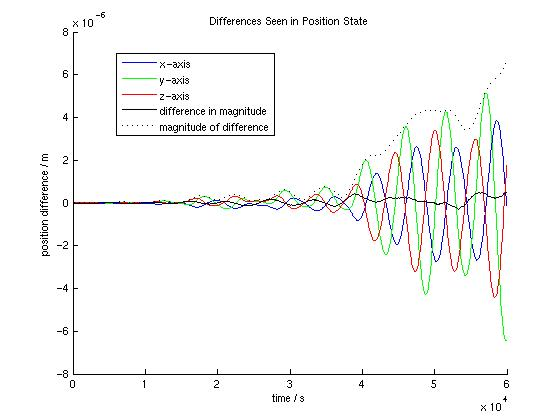
\includegraphics[width=3.2736in,height=2.85in]{figures/run1pos.jpg}
\caption{The difference in the position state for RUN\_1.}
\label{fig:sim71pos}
\end{center}
\end{figure}

\begin{figure}[htp]
\begin{center}
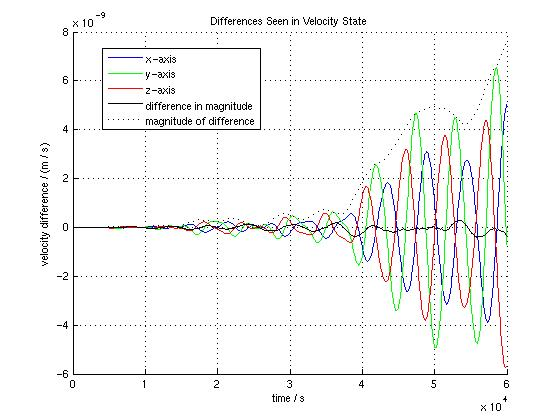
\includegraphics[width=3.2736in,height=2.85in]{figures/run1vel.jpg}
\caption{The difference in the velocity state for RUN\_1.}
\label{fig:sim71vel}
\end{center}
\end{figure}
 
\clearpage
{\bf RUN\_3A}
This run tests simple propagation in a nonspherical, 4x4 gravity field. 

The position diverges by centi-meters over the 120,000 seconds of the 
simulation (see figure \ref{fig:sim73apos}).

The velocity diverged by $O(10^{-5})$ meters per second (see figure 
\ref{fig:sim73avel}).


\begin{figure}[htp]
\begin{center}
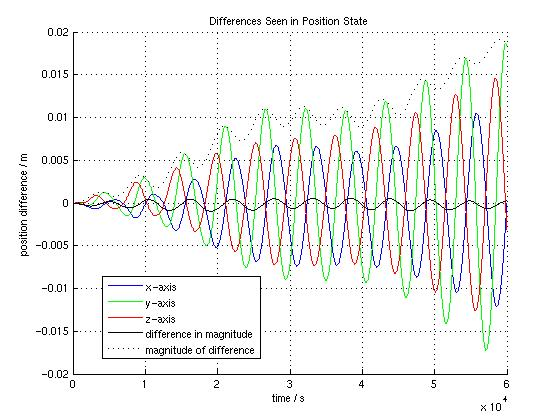
\includegraphics[width=3.2736in,height=2.85in]{figures/run3apos.jpg}
\caption{The difference in the position state for RUN\_3A.}
\label{fig:sim73apos}
\end{center}
\end{figure}

\begin{figure}[htp]
\begin{center}
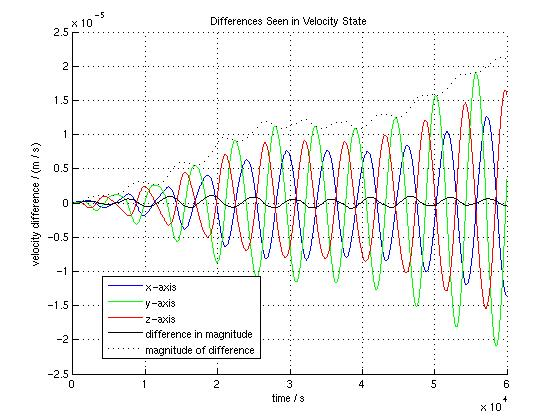
\includegraphics[width=3.2736in,height=2.85in]{figures/run3avel.jpg}
\caption{The difference in the velocity state for RUN\_3A.}
\label{fig:sim73avel}
\end{center}
\end{figure}



\clearpage
{\bf RUN\_3B}
This run tests simple propagation in a nonspherical, 8x8 gravity field. 

The position diverges by centimeters over the 120,000 seconds of the simulation 
(see figure \ref{fig:sim73bpos}).

The velocity diverged by $O(10^{-5})$ meters per second (see figure 
\ref{fig:sim73bvel}).


Because these data were significantly worse than the other simulations, we 
tried changing the rate at which the RNP matrix was being updated from once 
every 60 seconds to updates at 32 Hz, the same as the dynamic rate.  The 
rationale was demonstrated to have some validity, although the divergences in 
the enhanced state were still relatively large (see figures 
\ref{fig:sim73bhispdpos} and \ref{fig:sim73bhispdvel} for the enhanced 
simulation data).



\begin{figure}[htp]
\begin{center}
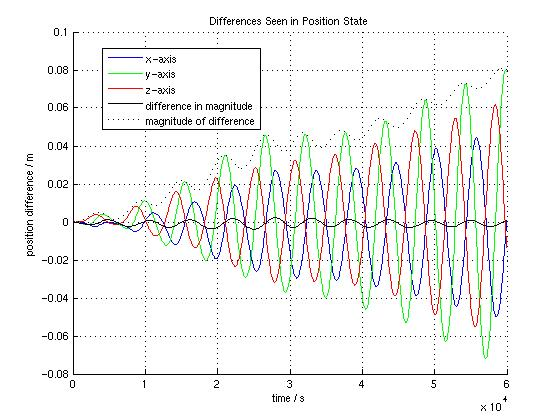
\includegraphics[width=3.2736in,height=2.85in]{figures/run3bpos.jpg}
\caption{The difference in the position state for RUN\_3B.}
\label{fig:sim73bpos}
\end{center}
\end{figure}

\begin{figure}[htp]
\begin{center}
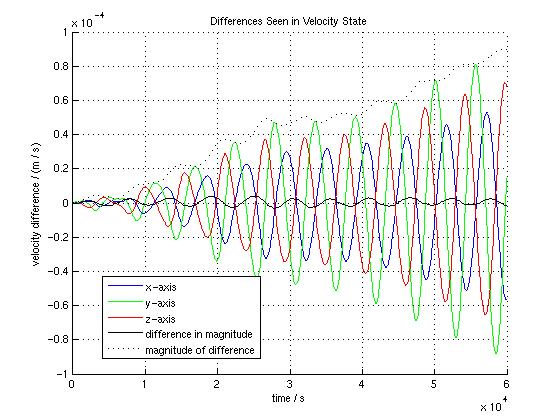
\includegraphics[width=3.2736in,height=2.85in]{figures/run3bvel.jpg}
\caption{The difference in the velocity state for RUN\_3B.}
\label{fig:sim73bvel}
\end{center}
\end{figure}

\begin{figure}[htp]
\begin{center}
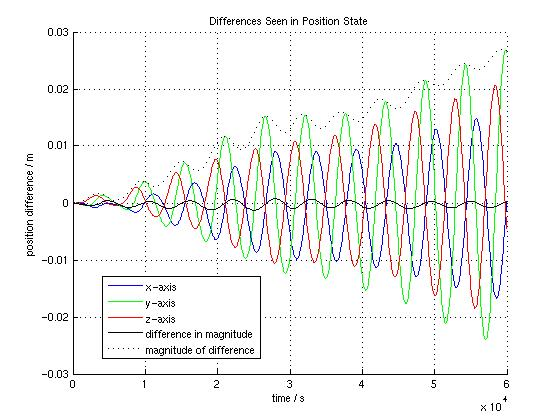
\includegraphics[width=3.2736in,height=2.85in]{figures/run_3bhispdpos.jpg}
\caption{The difference in the position state for RUN\_3B.}
\label{fig:sim73bhispdpos}
\end{center}
\end{figure}

\begin{figure}[htp]
\begin{center}
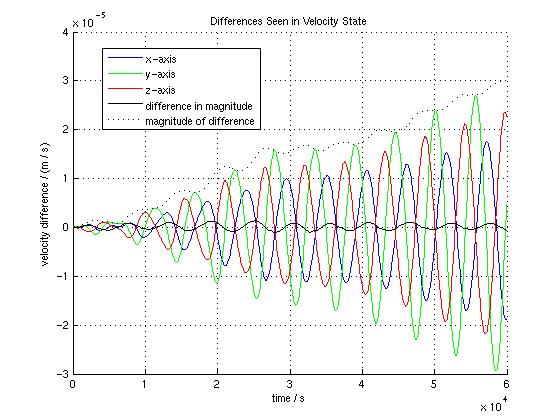
\includegraphics[width=3.2736in,height=2.85in]{figures/run_3bhispdvel.jpg}
\caption{The difference in the velocity state for RUN\_3B.}
\label{fig:sim73bhispdvel}
\end{center}
\end{figure}

\clearpage
{\bf RUN\_4}
This run tests propagation in a spherical gravitational field with 3rd body 
perturbations.

The position diverges by $O(10^{-5})$ meters over the 120,000 seconds of the
simulation (see figure \ref{fig:sim74pos}).

The velocity diverged by $O(10^{-8})$ meters per second (see figure
\ref{fig:sim74vel}).

\begin{figure}[htp]
\begin{center}
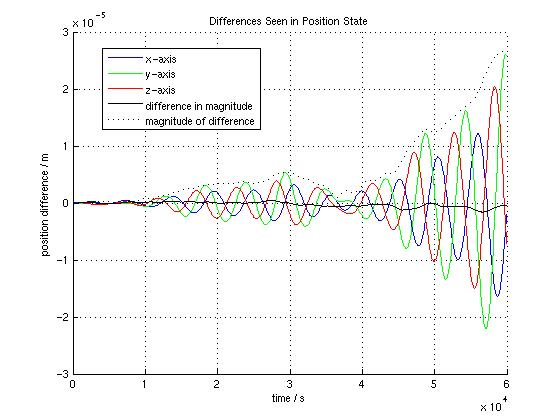
\includegraphics[width=3.2736in,height=2.85in]{figures/run4pos.jpg}
\caption{The difference in the position state for RUN\_4.}
\label{fig:sim74pos}
\end{center}
\end{figure}

\begin{figure}[htp]
\begin{center}
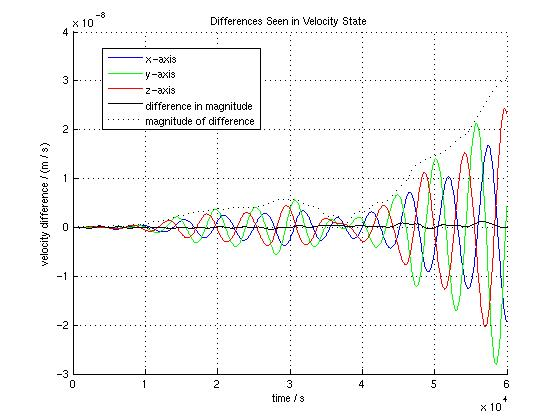
\includegraphics[width=3.2736in,height=2.85in]{figures/run4vel.jpg}
\caption{The difference in the velocity state for RUN\_4.}
\label{fig:sim74vel}
\end{center}
\end{figure}


\clearpage
{\bf RUN\_6A}
This run tests propagation in a spherical gravitational field with aerodynamic 
drag effects included.

The position diverges by $O(10^{-4})$ meters over the 120,000 seconds of the 
simulation (see figure \ref{fig:sim76apos}).

The velocity diverged by $O(10^{-7})$ meters per second (see figure 
\ref{fig:sim76avel}).

\begin{figure}[htp]
\begin{center}
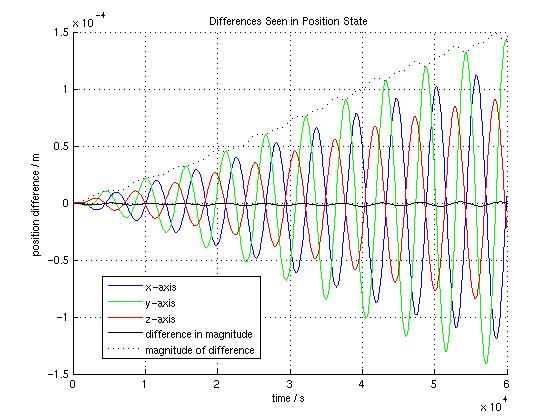
\includegraphics[width=3.2736in,height=2.85in]{figures/run6apos.jpg}
\caption{The difference in the position state for RUN\_6A.}
\label{fig:sim76apos}
\end{center}
\end{figure}

\begin{figure}[htp]
\begin{center}
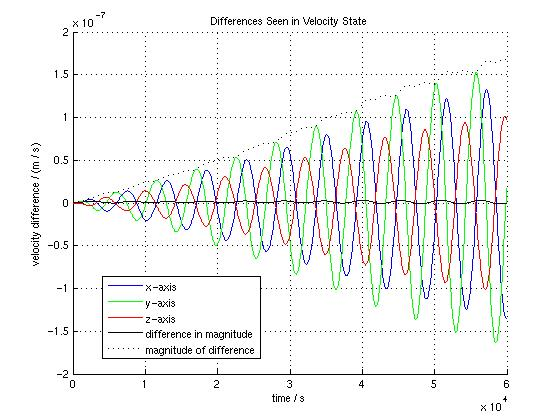
\includegraphics[width=3.2736in,height=2.85in]{figures/run6avel.jpg}
\caption{The difference in the velocity state for RUN\_6A.}
\label{fig:sim76avel}
\end{center}
\end{figure}

\clearpage
{\bf RUN\_8B}
This run tests propagation in a spherical gravitational field with the 
rotational state also available.  Only rotational data is provided here; the 
translational state is equivalent to that in RUN\_1.  RUN\_8B was chosen 
because it starts with a non-zero rotational state.

The quaternion values diverge by $O(10^{-14})$ over the 120,000 seconds of the 
simulation (see figure \ref{fig:sim78bpos}).

The angular velocity diverged by $O(10^{-14})$ radians per second (see figure 
\ref{fig:sim78bvel}).

\begin{figure}[htp]
\begin{center}
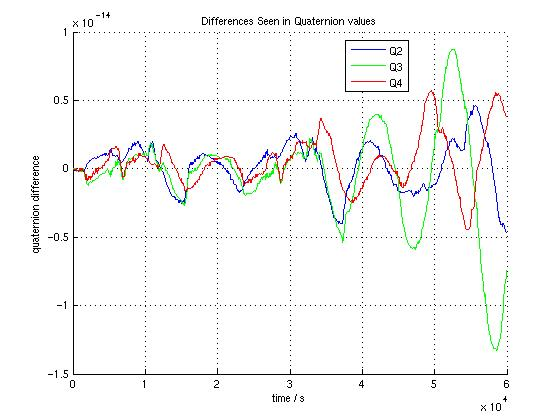
\includegraphics[width=3.2736in,height=2.85in]{figures/run8bpos.jpg}
\caption{The difference in the quaternion values for RUN\_8B.}
\label{fig:sim78bpos}
\end{center}
\end{figure}

\begin{figure}[htp]
\begin{center}
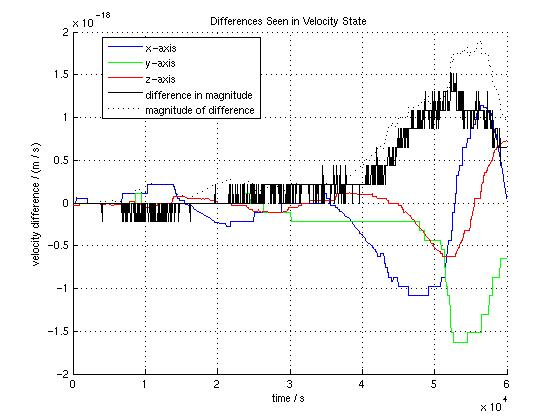
\includegraphics[width=3.2736in,height=2.85in]{figures/run8bvel.jpg}
\caption{The difference in the angular velocity state for RUN\_8B.}
\label{fig:sim78bvel}
\end{center}
\end{figure}

\clearpage
{\bf RUN\_9D}
This run tests propagation in a spherical gravitational field with rotational 
state and external torques and forces.  For this simulation, an external force 
and torque was applied between times t= 10,000 seconds and t = 20,000 seconds 
and then again between times t=100,000 seconds and t = 110,000 seconds to 
maintain the symmetry for the forward and reverse components.

The effect of the forces and torques on the state at the times for which they 
are active can be seen in figures \ref{fig:sim79dposoverall} and 
\ref{fig:sim79daveloverall}.

The position diverges by $O(10^{-7})$ meters over the 120,000 seconds of the 
simulation (see figure \ref{fig:sim79dpos}).

The velocity diverged by $O(10^{-10})$ meters per second (see figure 
\ref{fig:sim79dvel}).

The quaternion values diverge by $O(10^{-14})$ over the 120,000 seconds of the 
simulation (see figure \ref{fig:sim79dquat}).

The angular velocity diverged by $O(10^{-19})$ radians per second, at the limit 
of resolution (see figure \ref{fig:sim79davel}).


\begin{figure}[htp]
\begin{center}
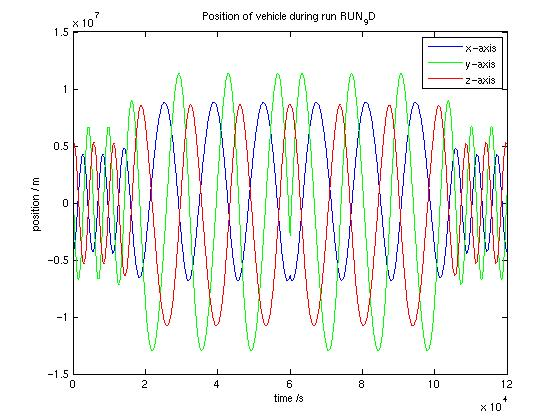
\includegraphics[width=3.2736in,height=2.85in]{figures/run_9dposoverall.jpg}
\caption{The position state for RUN\_9D.}
\label{fig:sim79dposoverall}
\end{center}
\end{figure}

\begin{figure}[htp]
\begin{center}
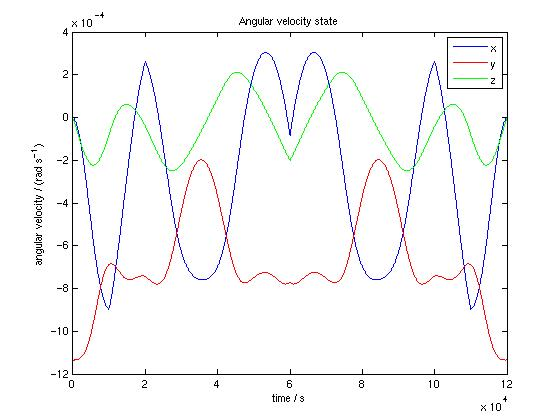
\includegraphics[width=3.2736in,height=2.85in]{figures/run_9daveloverall.jpg}
\caption{The angular velocity state for RUN\_9D.}
\label{fig:sim79daveloverall}
\end{center}
\end{figure}

\begin{figure}[htp]
\begin{center}
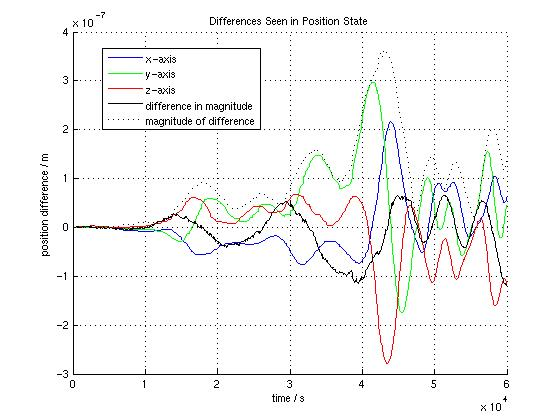
\includegraphics[width=3.2736in,height=2.85in]{figures/run_9dpos.jpg}
\caption{The difference in the position state for RUN\_9D.}
\label{fig:sim79dpos}
\end{center}
\end{figure}

\begin{figure}[htp]
\begin{center}
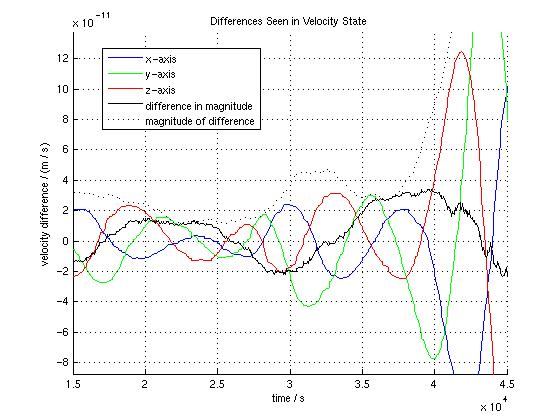
\includegraphics[width=3.2736in,height=2.85in]{figures/run_9dvel.jpg}
\caption{The difference in the velocity state for RUN\_9D.}
\label{fig:sim79dvel}
\end{center}
\end{figure}

\begin{figure}[htp]
\begin{center}
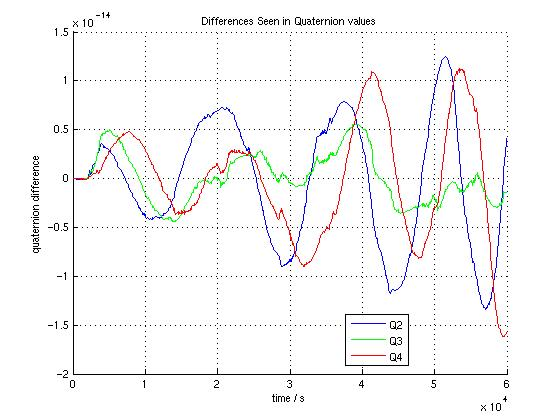
\includegraphics[width=3.2736in,height=2.85in]{figures/run_9dquat.jpg}
\caption{The difference in the quaternion values for RUN\_9D.}
\label{fig:sim79dquat}
\end{center}
\end{figure}

\begin{figure}[htp]
\begin{center}
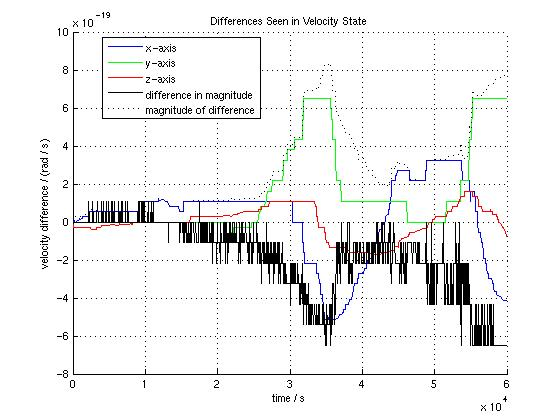
\includegraphics[width=3.2736in,height=2.85in]{figures/run_9davel.jpg}
\caption{The difference in the angular velocity state for RUN\_9D.}
\label{fig:sim79davel}
\end{center}
\end{figure}


\clearpage
{\bf RUN\_10A}
This final run tests propagation in a spherical gravitational field with 
gravity gradient torque present.

The position diverges by $O(10^{-6})$ meters over the 120,000 seconds of the 
simulation (see figure \ref{fig:sim710apos}).

The velocity diverged by $O(10^{-9})$ meters per second (see figure 
\ref{fig:sim710avel}).

The quaternion values diverge by $O(10^{-13})$ over the 120,000 seconds of the 
simulation (see figure \ref{fig:sim710aquat}).

The angular velocity diverged by $O(10^{-16})$ radians per second, at the limit 
of resolution (see figure \ref{fig:sim710aavel}).


\begin{figure}[htp]
\begin{center}
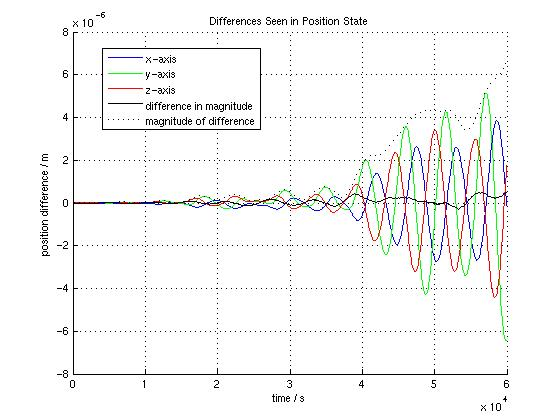
\includegraphics[width=3.2736in,height=2.85in]{figures/run_10apos.jpg}
\caption{The difference in the position state for RUN\_10A.}
\label{fig:sim710apos}
\end{center}
\end{figure}

\begin{figure}[htp]
\begin{center}
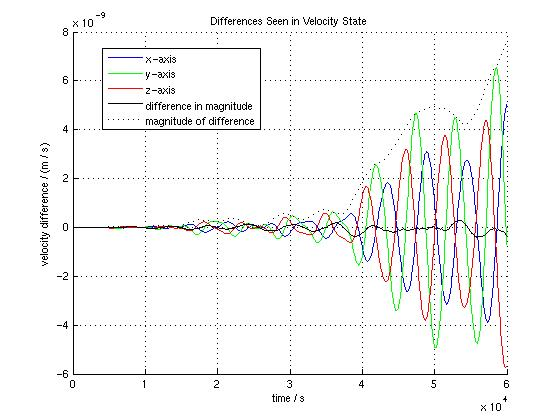
\includegraphics[width=3.2736in,height=2.85in]{figures/run_10avel.jpg}
\caption{The difference in the velocity state for RUN\_10A.}
\label{fig:sim710avel}
\end{center}
\end{figure}

\begin{figure}[htp]
\begin{center}
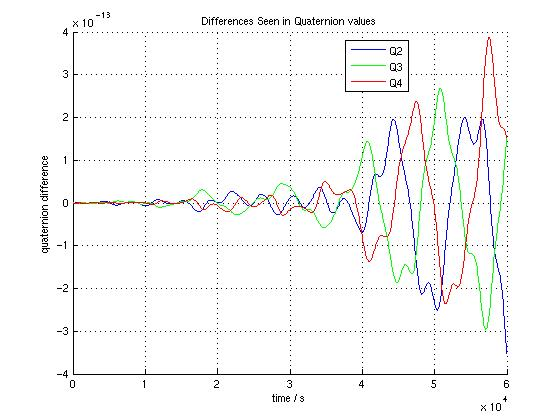
\includegraphics[width=3.2736in,height=2.85in]{figures/run_10aquat.jpg}
\caption{The difference in the quaternion values for RUN\_10A.}
\label{fig:sim710aquat}
\end{center}
\end{figure}

\begin{figure}[htp]
\begin{center}
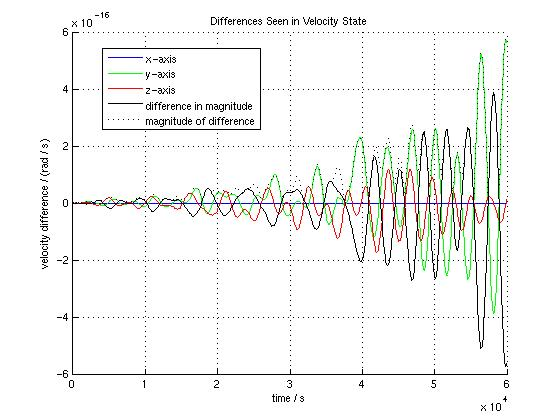
\includegraphics[width=3.2736in,height=2.85in]{figures/run_10aangvel.jpg}
\caption{The difference in the angular velocity state for RUN\_10A.}
\label{fig:sim710aavel}
\end{center}
\end{figure}

\end{description}
